\chapter{Project Design}

\section*{Introduction}
After having specified the project requirements in the  previous chapter, we are
going to present in the one,  the design of the Benchmarks Dashboard. To do so,
we will present the project global architecture. Finally, we will zoom into the
main layers of the project architecture and explain by providing the accurate
diagrams that describe it best.
\pagebreak

\section{UML}

\section{Mockups}
In this part we are going to describe and validate the project business
requirements in every UI views using mockups. First, we are going to present the
Pencil tool. Then we are going to define the project's mockups.

\subsection{Pencil}
Predictix development teams suggested to use Pencil, which is a small graphical
tool to sketch out use interfaces, for websites and web / desktop / mobile
application. Mockups provide enough interactivity to replace prototypes, and
make it easy to collaborate and get feedback on the wireframes.

\subsection{Project mockups}
In this section, we are going to describe our project's components mockups.

UI general Description

The Benchmarks dashboard is composed of five main screens which are the account
choice, Account's info, Tests choice, Test, New Benchmarks. In the following,
we are going to proceed by describing the mockups and the need required in every
view.

\subsection{Account choice}
The figure
\hyperref[fig:benchmarks_dashboard_home]{\ref{fig:benchmarks_dashboard_home}}
represents the landing page of our application, for a administrator user,
after the authentication screen which the account's choice. The page should
contain a list of the different accounts that the user have access to. In fact,
the user should have the possibility to select a certain account, in order to
view the all benchmarks run and the list of tests of that project.

\begin{figure}[ht]
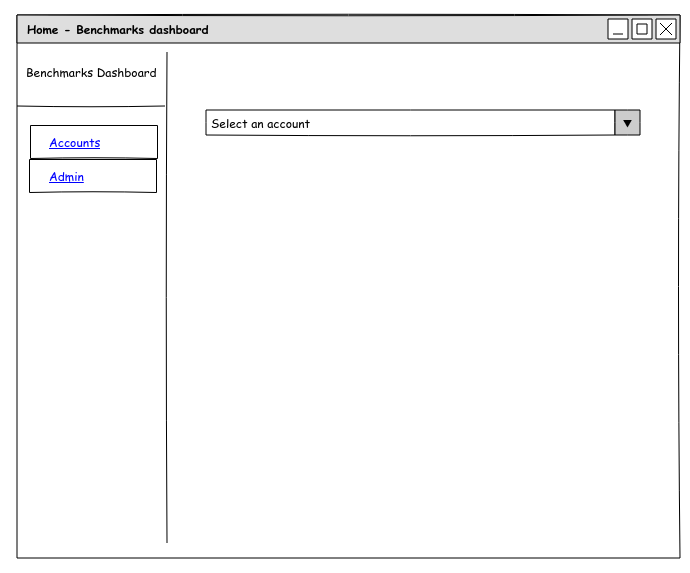
\includegraphics[width=15cm]{home}
\caption{Benchmarks dashboard Home}
\label{fig:benchmarks_dashboard_home}
\end{figure}

\subsection{Account overview}
\hyperref[fig:benchmarks_dashboard_overview]{\ref{fig:benchmarks_dashboard_overview}}
represents the Account overview screen mockup. This page is generated after a
user selected an account. This page will contain a chart that represent the
overall performance of the account's tests. The chart will contain the total
duration it took every benchmark run to finish. It will give a general overview
on the state of the account's applications, the general trend for its tests and
also any alerts about the the current benchmarks status.

\begin{figure}[ht]
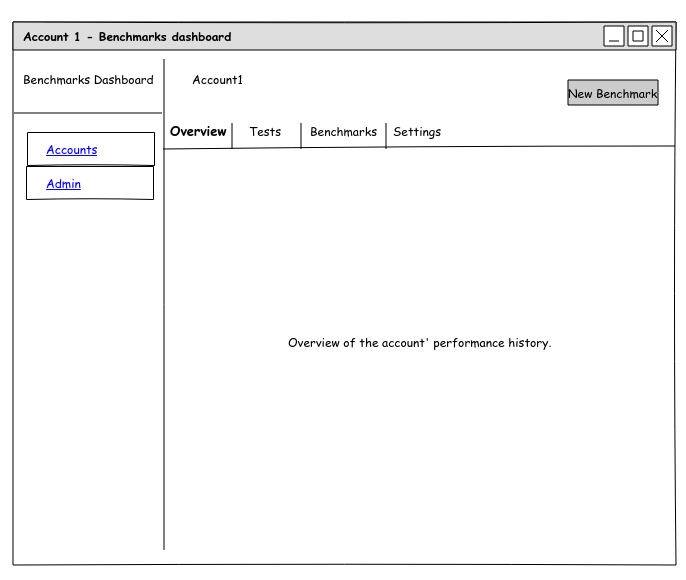
\includegraphics[width=15cm]{overview}
\caption{Account overview}
\label{fig:benchmarks_dashboard_overview}
\end{figure}

\subsection{New deployment}
The figure
\hyperref[fig:benchmarks_dashboard_home]{\ref{fig:benchmarks_dashboard_home}}
represents the landing page of our application, for a administrator user,
after the authentication screen which the account's choice. The page should
contain a list of the different accounts that the user have access to. In fact,
the user should have the possibility to select a certain account, in order to
view the all benchmarks run and the list of tests of that project.

\begin{figure}[ht]
  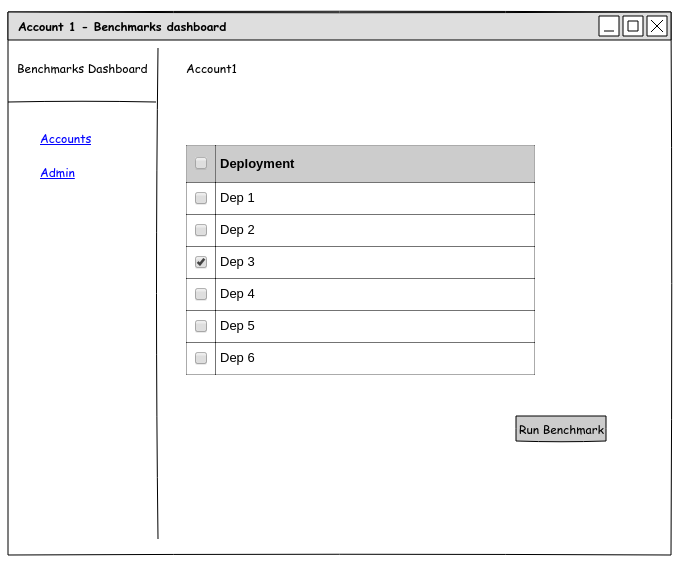
\includegraphics[width=15cm]{deployments}
  \caption{New benchmark screen}
\label{fig:benchmarks_dashboard_home}
\end{figure}

\subsection{Account' tests}
\hyperref[fig:benchmarks_dashboard_tests]{\ref{fig:benchmarks_dashboard_tests}}
represents the account's tests mockup. This screen will present the list of all
account's tests. This list will show the test name, the percentage of time
difference between the latest two runs for that test and the difference in
seconds. The list tests that exceed 15 seconds in difference will be highlighted
in red and those that exceed 5 seconds will be highlighted in yellow. This will
help the user to identify malfunctioning tests. Th

\begin{figure}[ht]
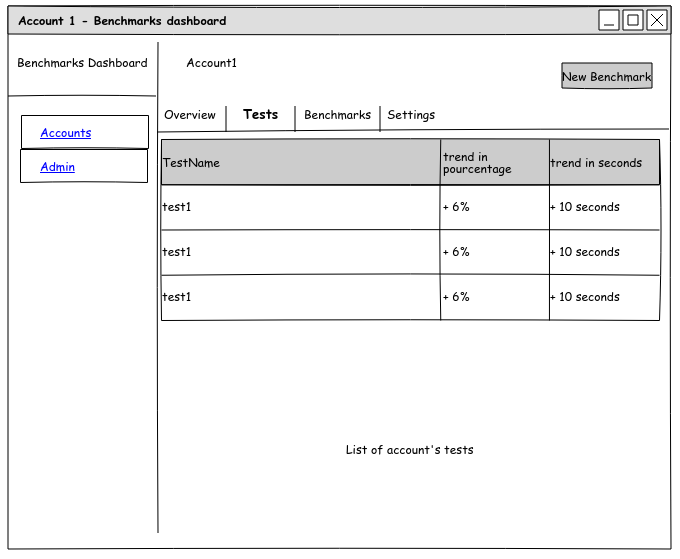
\includegraphics[width=15cm]{tests}
\caption{Account overview}
\label{fig:benchmarks_dashboard_tests}
\end{figure}

